% &pdflatex
\documentclass[11pt, a4paper]{article}
\usepackage{graphicx}
\usepackage{amsmath}
\usepackage{listings}
\usepackage{minted}
\usepackage{float}
\usepackage{algorithmic}
\usepackage{hyperref}
\hypersetup{
    colorlinks=true,
    linkcolor=blue,
    filecolor=magenta,      
    urlcolor=cyan,
}

\title{EE2703 Applied Programming Lab - \\Final Assignment}
\author{
  \textbf{Name}: Abishek S\\
  \textbf{Roll Number}: EE18B001
}\date{\today}

\begin{document}
		
\maketitle 

\section{Abstract}
The goal of this assignment is the following :
\begin{itemize}
\item To model a rectangular tank filled with dielectric fluid as a capacitor.
\item To solve 2-D Laplace equation numerically in an iterative manner using vectorised code.
\item To develop an algorithm to calculate height of fluid in tank given the resonant frequency.
\item To estimate electric field from the potential matrix.
\item To observe the variation of $Q_{top}$ and $Q_{fluid}$ Vs $h$.
\item To check continuity of normal electric displacement ($D_n$) at the fluid's top surface.
\item To check the validity of snell's law for electric field at the fluid's top surface.
\end{itemize}
\usemintedstyle{manni}

\section{Assignment}
The 2-D Laplace equation is :
\begin{equation*}
\nabla^2\phi = 0
\end{equation*}
\begin{center}
\textbf{OR}
\end{center}
\begin{equation*}
\frac{\partial^2\phi}{\partial x^2} + \frac{\partial^2\phi}{\partial y^2} = 0
\end{equation*}
The above combined with handling continuity of $D_n$ at the fluid-air interface (m = k) gives rise to the following equations :
\begin{equation*}\label{eq:1}
\begin{aligned}[c]
  \phi_{m,n} = \frac{\phi_{m-1,n} + \phi_{m+1,n} + \phi_{m,n-1} + \phi_{m,n+1}}{4}
  \\
  \phi_{k,n} = \frac{\epsilon_r\phi_{k-1,n} + \phi_{k+1,n}}{1 + \epsilon_r}
\end{aligned} 
\hspace{0.1in}  
\begin{aligned}[c]
  m \neq k,0 < m < M,0 < n < N 
  \\
  \\
  m = k,0 < n < N 
\end{aligned} 
\end{equation*}
\\

\subsection{Setting up the program and configuring parameters}
Importing necessary libraries
\begin{minted}[tabsize = 4]{python3}
import pylab as pl
import argparse
from scipy.linalg import lstsq
import sys
import matplotlib
\end{minted}
Getting optional arguments from the user using argparse for configuring the parameters
\begin{minted}[tabsize = 4]{python3}
parser.add_argument('--M',dest='M',type=int,default=41, 
  help = 'The number of nodes along y, including the boundary nodes (>= 2)')
parser.add_argument('--N',dest='N',type=int,default=21,  
  help = 'The number of nodes along x, including the boundary nodes) (>= 2)')
parser.add_argument('--delta',dest='delta',type=float,default=1e-8, 
  help = 'The desired accuracy for the potential obtained')
parser.add_argument('--Ni',dest='NIter_max',type=int,default=3000, 
  help = 'The maximum number of iterations to complete for convergence')

args = parser.parse_args()
M,N,delta,NIter_max = args.M,args.N,args.delta,args.NIter_max
\end{minted}
Also initialising or calculating other parameters needed for the program to run 
\begin{minted}[tabsize = 4]{python3}
'''
  Lx : 10 cm - Physical length of tank along x direction
  Ly : 20 cm - Physical length of tank along y direction
  e_r : 2 - Relative permttivity of fluid in tank
'''
Lx,Ly,e_r = 0.1, 0.2, 2.0  # Lx, Ly in metres

# Checking if distance between a node is same along x and along y
if (Ly / (M-1)) != (Lx / (N-1)):
    print('\nMake sure ditance between nodes along x and along y \
      are equal for given M and N')
    sys.exit()

# Distance between nodes (same along x and along y) in metres
dist = Ly / (M-1)

EPS = 1e-9 # A constant to compare equal decimals 
#   which would differ slightly due to machine precision
e_o = 8.854e-12 # Absolute Pe_rmittivity of free space - constant
\end{minted}
Defining a utility function to make plotting easier since it is used a lot :
\begin{minted}[tabsize = 4]{python3}
  def PLOT(x,y,label_x = r'X$\rightarrow$',label_y = r'Y$\rightarrow$',
    fn = pl.plot,arg3 = '-',title = "Plot",fig_no = 0,grids = True,
    label = '',cmap = matplotlib.cm.jet):
  '''
      Utility function for making the more repeated plots
      Takes in -
          x : Data points for x axis
          y  : Data points for y axis
          label_x : Label for x axis
          label_y : Label for y axis
          fn : Which plot function to use
          arg3 : 3rd  argument to the function - 
            (the matrix for contour plot, the line style for normal plot)
          title : Title for the plot
          fig_no : Figure number for the plot
          grids : True is grids need to be present on the plot, False otherwise
          label : Legend label for the plot drawn
          cmap : Colour map to use for the contour plot
  '''
  pl.figure(fig_no)
  if fn == pl.contourf:
      fn(x,y,arg3,cmap = cmap)
      pl.colorbar()
  else:
      if label == '':
          fn(x,y,arg3)
      else:
          fn(x,y,arg3,label = label)
  pl.xlabel(label_x,size=15)
  pl.ylabel(label_y,size=15)
  pl.title(title,size=16)
  pl.grid(grids)
\end{minted}

\subsection{Part B - My Algorithm to find \textit{h} from resonant frequency}
Let's look at $Q_{top}$ Vs $h$ plot that we got \hyperref[fig:qtop]{here}. The plot isn't linear clearly, neither is it exponential nor a simple hyperbolic (without shifting in Q direction)
as can be seen \hyperref[fig:qtop_semilog]{here}. The plot appears like it can be interploated with polynomials (it can also be a shifted hyperbola like in simple parallel plate capacitors, but then since $Q << 1$, using taylor's series we can get polynomials to fit the curve with minimal error).
\\
We have the data points as we ran the program for a range of h values. The plot points can be interpolated by \textbf{Numerical methods for polynomial interpolation} like \textbf{Newton's method or spline method}.
The points are indeed interpolated by linear spline in the plot, but using a quadratic or cubic spline (if polynomial doesn't fit the entire curve well, in which case we can fit each range by a different polynomial), or Newton's method (if a polynomial fits well) can give smooth and more accurate curves.
We can even use polynomial regression as in supervised learning to fit a polynomial, but since the data points are small in number, neglecting it.
\\ \\
Suppose we need value of h, given Q. Another important observation from the plot is that it is monotonically increasing, which implies we can use \textbf{Binary Search}.
Thus, once we obtain a reasonable polynomial fit for the data points we can binary search for the value of h to the required precision.
\\ \\
All this done because we can get the value of capacitance of this tank, once we know the resonant frequency and the inductance value (resistance value won't affect the resonant frequency).
Since we know the value of potential across the capacitor (which is 1V here), we can get Q from the formula $Q = CV$. 
From Q, we estimate h.
\\ \\
Formally put, the algorithm is :
\begin{algorithmic}
\STATE For series RLC circuit $f_{res} = \frac{1}{2\pi\sqrt{LC}}$

\STATE $Given\ V,L,f_{res}$
\STATE $C \gets \frac{1}{4 \pi^2 f_{res}^2 L}$
\vspace{0.1in}
\STATE $Q \gets CV$

\STATE Let polynomial fit obtained for $Q$ Vs $h$ be $p(x)$ 
\STATE $h \gets binary\_search(p,Q)$
\end{algorithmic}
where $binary\_search(p,Q)$ searches for $x_o \mid p(x_o) = Q$ in $\mathcal{O}(\log n)$
($n$ is the range to search times the precision required)

\subsection{Part C - Parallelising the computation}
I use vectorised code and avoid loops wherever possible. A few examples :
\begin{minted}[tabsize = 4]{python3}
for iter_no in range(Ni_max):
      Ni += 1
      oldPhi = phi.copy()
      ##### Using vectorised code to execute code faster #####
      # Interior Points from 0 to (k-1)th index - average of surrounding points
      phi[1:k,1:-1] = 0.25 * (oldPhi[0:k-1,1:-1] + 
        oldPhi[2:k+1,1:-1] + oldPhi[1:k,0:-2] + oldPhi[1:k,2:])
      # Interior Points from (k+1)th to Nth index - average of surrounding points
      phi[k+1:-1,1:-1] = 0.25 * (oldPhi[k:-2,1:-1] + oldPhi[k+2:,1:-1] +
        oldPhi[k+1:-1,0:-2] + oldPhi[k+1:-1,2:])
      # Interior Points at kth index - slightly different updation 
      # to handle Dn continuity
      global e_r
      phi[k,1:-1] = (e_r*oldPhi[k-1,1:-1] + oldPhi[k+1,1:-1]) / (1 + e_r)

      # The top, bottom and side boundaries are at constant potentials
      # as initialised and unaffected by above update
      # Hence not running below code and increase the time taken
      # phi[0,:] = 0  # Bottom side
      # phi[:,0] = 0  # Left side
      # phi[:,-1] = 0  #Right side
      # phi[-1,1:-1] = 1  # Top side
\end{minted}
The above snippet is from \hyperref[lst:laplace_solver]{potential updation in laplace solver}. Since m = k row is handled differently,
I break the whole matrix into three parts and use vectorised code on each part to make computations faster. Also, I don't update the boundary points explicitly 
since the boundary points are never disturbed in a updation and stays in the same value it was initialised with (where I assign the proper values).
The optimisation though is very specific to this problem, since the boundary points are at constant potential, but such small things might matter 
if the code is to be run for many iterations, and the size of M and N becomes larger.
\\
Apart from the above, we can also see that the rows from 1 to k-1 and k to M-1 are handled by the same formula above.
So instead of sequentially updating those two sets of rows, we can use \textbf{multithreading} or \textbf{multiprocessing} to update them parallely.
\\
\begin{minted}[tabsize = 4]{python3}
Ex[:,1:] = -(phi[:,1:] - phi[:,:-1]) / dist
Ey[1:,:] = -(phi[1:,:] - phi[:-1,:]) / dist
\end{minted}
The above is another small example from \hyperref[lst:EF]{electric field calculation}. There are many such examples in this program wherever I use numeric gradient or updation.
\\ \\
Vectorisation of code is so important a topic nowadays when using such numeric and iterative methods, because of improvement in efficiency it offers.
Loops are quite a overhead, especially in interpreted languages like Python which increases computing time considerably.
Since the \textbf{Numeric Python} (NumPy, in short) library is written in C, the vectorised methods offer a significant improvement in efficiency over loops.
Also some libraries in Python and other languages developed for doing numeric calculations use the parallelism offered by computers having many CPUs or atleast many CPU cores
to improve the performance the vectorised code.

\subsection{Part D - Solving the Laplace Equation}
We iteratively keep updating the potential grid usinng the previous iteration values according to the formula given \hyperref[eq:1]{here},
till the value converges (i.e) the difference between previous and present value goes below a $\delta$ (denoted by accuracy here).
\\ The function for doing the above mentioned operation is given below :
\\
\begin{minted}[tabsize = 4]{python3}
  def solveLaplace(M,N,dist,k,delta,Ni_max):
  ''' 
      The function solves Laplace equation given -
          M : The number of nodes along y, including the boundary nodes
          N : The number of nodes along x, including the boundary nodes
          dist : Distance between nodes (same along x and along y)
          k : The height given as the index k corresponding to h
          delta : The desired accuracy for the potential obtained
          Ni_max : The maximum number of iterations to complete for convergence
      -----------------------------------------------
      The function returns -
          phi[M,N] : The array of solved potential values correct to delta
          Ni : Number of iterations actually carried out
          err[Ni] : The vector of errors
  '''
  # phi is a matrix where (0,0) corresponds to the lower left corner of tank 
    and (M-1,N-1) corresponds to the top right corner
  phi = pl.zeros(shape = (M,N)) # Initialising Potential grid to zero at all nodes
  phi[-1,1:-1] = 1 # Top boundary points are at 1V
  # The bottom and side boundary points are at 0 V (grounded)
  # which is already satisfied
  errors = pl.zeros(Ni_max)
  Ni = 0

  for iter_no in range(Ni_max):
      Ni += 1
      oldPhi = phi.copy()
      ##### Using vectorised code to execute code faster #####
      # Interior Points from 0 to (k-1)th index - average of surrounding points
      phi[1:k,1:-1] = 0.25 * (oldPhi[0:k-1,1:-1] + 
        oldPhi[2:k+1,1:-1] + oldPhi[1:k,0:-2] + oldPhi[1:k,2:])
      # Interior Points from (k+1)th to Nth index - average of surrounding points
      phi[k+1:-1,1:-1] = 0.25 * (oldPhi[k:-2,1:-1] + oldPhi[k+2:,1:-1] +
        oldPhi[k+1:-1,0:-2] + oldPhi[k+1:-1,2:])
      # Interior Points at kth index - slightly different updation 
      # to handle Dn continuity
      global e_r
      phi[k,1:-1] = (e_r*oldPhi[k-1,1:-1] + oldPhi[k+1,1:-1]) / (1 + e_r)

      # The top, bottom and side boundaries are at constant potentials
      # as initialised and unaffected by above update
      # Hence not running below code and increase the time taken
      # phi[0,:] = 0  # Bottom side
      # phi[:,0] = 0  # Left side
      # phi[:,-1] = 0  #Right side
      # phi[-1,1:-1] = 1  # Top side
      
      errors[iter_no] = (abs(phi-oldPhi)).max()
      if iter_no > 500 and errors[iter_no] < delta:
          # Running minimum 500 iterations to get a fitting for the error
          # after 500 iterations
          # Exiting the iterations on reaching desired accuracy
          # (i.e) when error goes below the required limit
          break
  
  errors = errors[:Ni]
  return phi,Ni,errors
\end{minted}
\label{lst:laplace_solver}

\subsection{Part E - Solve Laplace Equation for different \textit{h} values}
We define two functions, one for calculating the Electric Fields along x direction at points (m,n+0.5) and y direction at points (m+0.5,n), using one-sided numerical derivative
and the other for calculating $Q_{top}$ and $Q_{fluid}$.
\begin{minted}[tabsize = 4]{python3}
def ElectricField(phi):
  '''
      Function to calculate electric field along x and y directions 
        using one sided derivative
      Takes in -
          phi : The potential grid
      -----------------------------------------------
      Returns - 
          Ex : Electric field along x direction {Ex[m,n] for points (m,n-0.5)  
            - since one sided derivative used}
          Ey : Electric field along y direction {Ey[m,n] for points (m-0.5,n) 
            - since one sided derivative used}
  '''
  global dist
  Ex = pl.zeros((M,N))
  Ey = pl.zeros((M,N))

  # Electric field is calculated as numerical one-sided derivative of potential 
  # along respective directions
  # Ex[i,j+1] = -(phi[i,j+1] - phi[i,j]) / dist 
  # and Ey[i+1,j] = -(phi[i+1,j] - phi[i,j]) / dist
  # where dist = delta x = delta y
  Ex[:,1:] = -(phi[:,1:] - phi[:,:-1]) / dist
  Ey[1:,:] = -(phi[1:,:] - phi[:-1,:]) / dist

  return Ex,Ey


def Charge_Top_Fluid(Ex,Ey):
  '''
      Function to caclulate Qtop and Qfluid
      Takes in -
          Ex : Electric field along x direction at (m,n+0.5)
          Ey : Electric field along y direction at (m+0.5,n)
      -----------------------------------------------
      Returns -
          Qtop : Charge at the top surface
          Qfluid : Charge at the surfaces in contact with the fluid
  '''
  # En_top is normal electric field (along +y direction - outward normal)  
  # at the top surface (i.e) (M-0.5,n)
  En_top = Ey[-1,:]
  # En_lside is normal electric field (along -x direction - outward normal)  
  # at the left side till fluid is present (i.e) (m,0.5)
  En_lside = -Ex[:k+1,1]
  # En_rside is normal electric field (along +x direction - outward normal)  
  # at the right side till fluid is present (i.e) (m,N-0.5)
  En_rside = Ex[:k+1,-1]
  # En_bottom is normal electric field (along -y direction - outward normal) 
  # at the bottom surface (i.e) (0.5,n)
  En_bottom = -Ey[1,:]

  global e_o,e_r,dist

  # Qtop consists of only the top wall
  Qtop = -e_o * sum(En_top) * dist  
  # dist is constant over summation hence brought out 

  # Qfluid consists of the side walls till height h and the bottom wall
  Qfluid = -e_o*e_r * (sum(En_lside) + sum(En_rside) + sum(En_bottom)) * dist  
  # dist is constant over summation hence brought out 

  return Qtop,Qfluid
\end{minted}
\label{lst:EF}

We run the laplace equation solver for differernt values of h - specifically, for $\frac{h}{L_y} = 0.1,0.2,...,0.9$.
\\
\textit{\textbf{k}} as we know is the index of the fluid surface, that is the y-index in grid corresponding to height \textit{\textbf{h}}.
We make sure that there exists an integer index \textit{\textbf{k}} corresponding to the \textit{\textbf{h}}, and then run the laplace equation solver for it.
\\ \\
From the solved laplace equation, we can plot potential contours. I have also tried to fit an exponential for the error as $y = Ae^{Bx}$,
where $y$ is the error and $x$ is the iteration number, after 500 iterations (after which the semilogy plot goes into the linear regime).
Using this estimated error, we can then extrapolate the error to $\infty$ and obtain the cumulative error after the current number of iterations the potential grid went through.
The formula for the cumulative error after the N interations extrapolated to $\infty$ is given by :
\[
  Error = \sum_{i=N+1}^{\infty} error_i
  \\
    < \sum_{i=N+1}^{\infty} Ae^{Bi}
  \\
    \approx \int_{N+0.5}^{\infty} Ae^{Bx} \,\mathrm{d}x 
  \\
    = -\frac{A}{B}exp(B(N+0.5))
\]

\begin{minted}[tabsize = 4]{python3}
# x and y are the axes of the grid to make the contour plot
x = pl.linspace(0,Lx,N)*100  # in cm
y = pl.linspace(0,Ly,M)*100  # in cm

# Qtop is the charge on the top plate
Qtop = pl.zeros(9)
# Qfluid is the charge on the walls of tank in contact with the fluid
Qfluid = pl.zeros(9)

for ind,hbyLy in enumerate([x*0.1 for x in range(1,10)]):
    # h/Ly = k/(M-1) but k and M are integers => (h*(M-1)/Ly) should be an integer
    k = (hbyLy*(M-1))
    if abs(k - int(k)) > EPS:
        # k is not an integer
        print("\nFor the given value of M and h, \
          there doesn't exist an index corresponding to the fluid top boundary")
        sys.exit()
    k = int(k)
    phi,Ni,errors = solveLaplace(M,N,dist,k,delta,NIter_max)
    # Fitting an exponential to the error obtained during each iteration
    # Obtaining A and B by using lstsq on log(y) = log(A) + B.x,  
    # where y is error and x is the iteration number
    A,B = lstsq(pl.c_[pl.ones(Ni-499),pl.arange(500,Ni+1)],pl.log(errors[499:]))[0]
    A = pl.exp(A)
    print('\nThe values of A and B for which Ae^(Bk) fits the  \
      iteration error vector (for h/Ly = {:.1f}):'.format(hbyLy))
    print(A,B)
    print('The maximum error on extrapolating the error to infinity \
      (for h/Ly = {:.1f}):'.format(hbyLy))
    print(-A/B * pl.exp(B*(Ni+0.5)))
    # The exponential which fits the iteration error
    error_fit = A * pl.exp(B*pl.arange(500,Ni+1))

    # Uncomment the below lines to view the potential contour plots 
    # and semilog plot of error with the extrapolation
    # PLOT(pl.arange(1,Ni+1),errors,r'$Number\ of\ iterations\rightarrow$' 
      ,r'$Error\rightarrow$',pl.semilogy,'b-',r'$Log\ (error)\ vs\ Iteration\
      number\ for\ h/L_y\ =\ {:.1f}$'.format(hbyLy),0,True,'True iteration error')
    # #pl.semilogy(pl.arange(500,Ni+1),error_fit,'g-',label = 'Fitted error')
    # pl.legend()
    # pl.show()
    # PLOT(x,y,r'$X\ (in\ cm)\ \rightarrow$',r'$Y\ (in\ cm)\ \rightarrow$',  
      pl.contourf,phi,r'$Contour\ plot\ of\ Potential\ for\ h/L_y\ =\ 
      {:.1f}$'.format(hbyLy),1,cmap = matplotlib.cm.plasma)
    # pl.show()

    '''
        Since the walls of the tank are all made of conductors, we can use 
          the fact that -D.n = sigma
        where n - the outward normal to the wall at a point and sigma - 
          the charge density (charge/unit area) at that point

        Hence we can sum the sigma multiplied by dist (numerically equal 
          to the small length over which sigma is the charge density) 
          at each point to get charge per unit depth of the tank
        Q = charge over unit depth (depth of tank (Lz) is unknown and constant
          so we can assume it is unity(1 metre) )
    '''
    # D.n can be calculated as -e dV/dn where e is absolute permittivity
    # of medium = e_o * e_r, dV/dn is derivative of potential along 
    # outward normal direction
    # We use numerical approximation on derivative => dv = V[i+1] - V[i] 
    # and dn = dist = delta x = delta y

    Ex,Ey = ElectricField(phi)
    Qtop[ind],Qfluid[ind] = Charge_Top_Fluid(Ex,Ey)
\end{minted}
I show one contour plot of the potential matrix and the iteration error plot here as an example :
\begin{figure}[H]
   	\centering
   	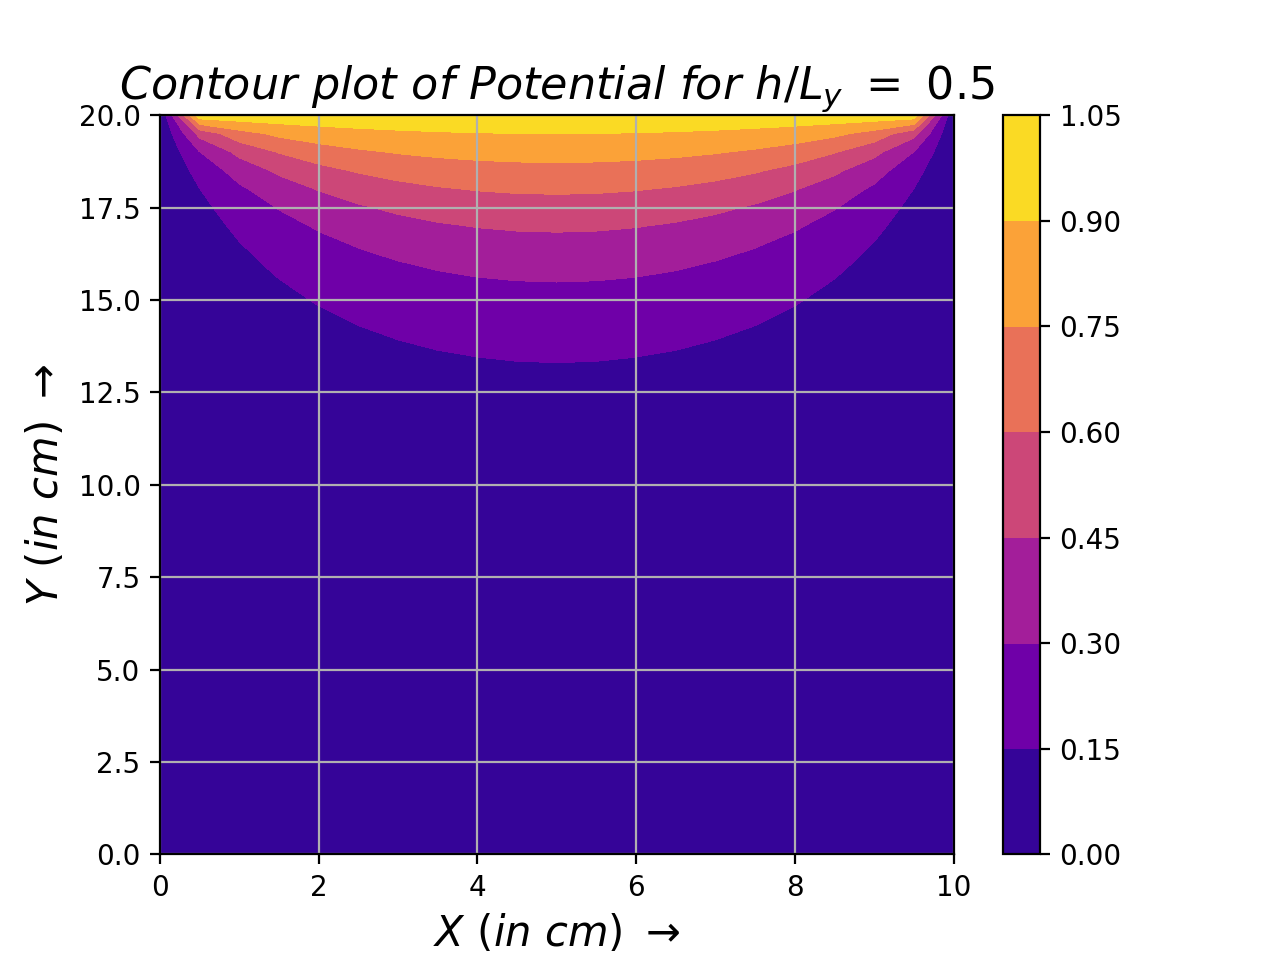
\includegraphics[scale=0.6]{cont_potl.png}
   	\label{fig:cont_potl}
   	\caption{Contour plot of Potential}
\end{figure}
\begin{figure}[H]
   	\centering
   	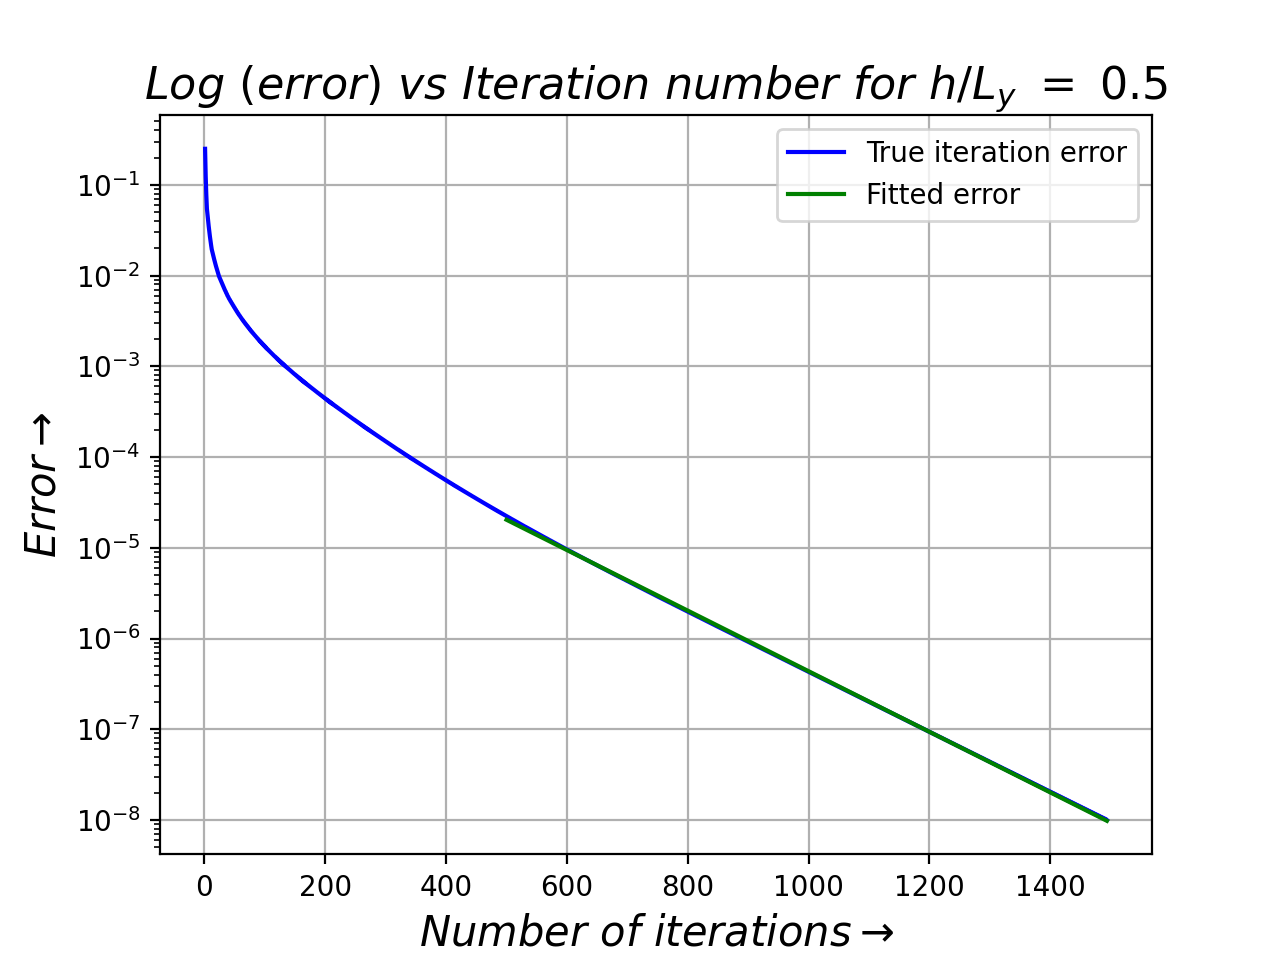
\includegraphics[scale=0.6]{iter_error.png}
   	\label{fig:iter_error}
   	\caption{Error vs Iteration - Semilogy plot}
\end{figure}
\begin{figure}[H]
   	\centering
   	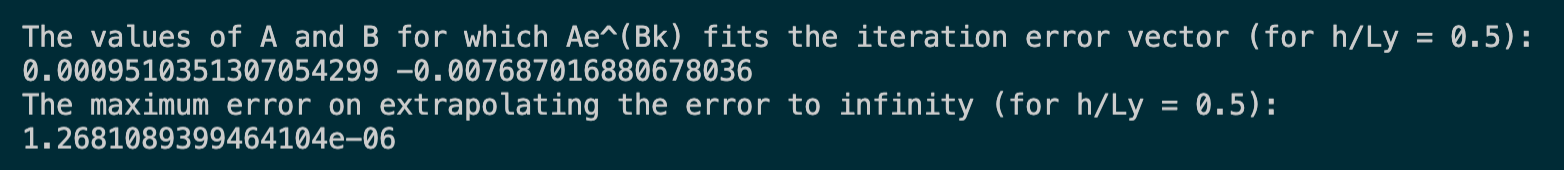
\includegraphics[scale=0.5]{error_fit.png}
   	\label{fig:error_fit}
   	\caption{Screenshot of output on Error fitting}
\end{figure}
The $Q_{top}$ and $Q_{fluid}$ was calculated from the following boundary condition equation for conductors :
\[
  -D.\hat{n} = \sigma
  \\ \implies 
  \int (-D.\hat{n}) \,\mathrm{d}A
  \\ \approx
  \sum (-D.\hat{n})\Delta A = Q 
\]
where D is the Electric Displacement vector and $\hat{n}$ is along outward normal.
\\
For $Q_{fluid}$ the side walls (upto the fluid's top surface) and the bottom walls are considered, whereas for $Q_{top}$ the top wall alone is considered.
\\
\indent$\Delta A = 1.\Delta l$, since I assume Lz = depth of tank as $1\ metre$
\\ \\
The plots $Q_{fluid}$ vs h and $Q_{top}$ vs h are drawn :
\begin{figure}[H]
  \centering
  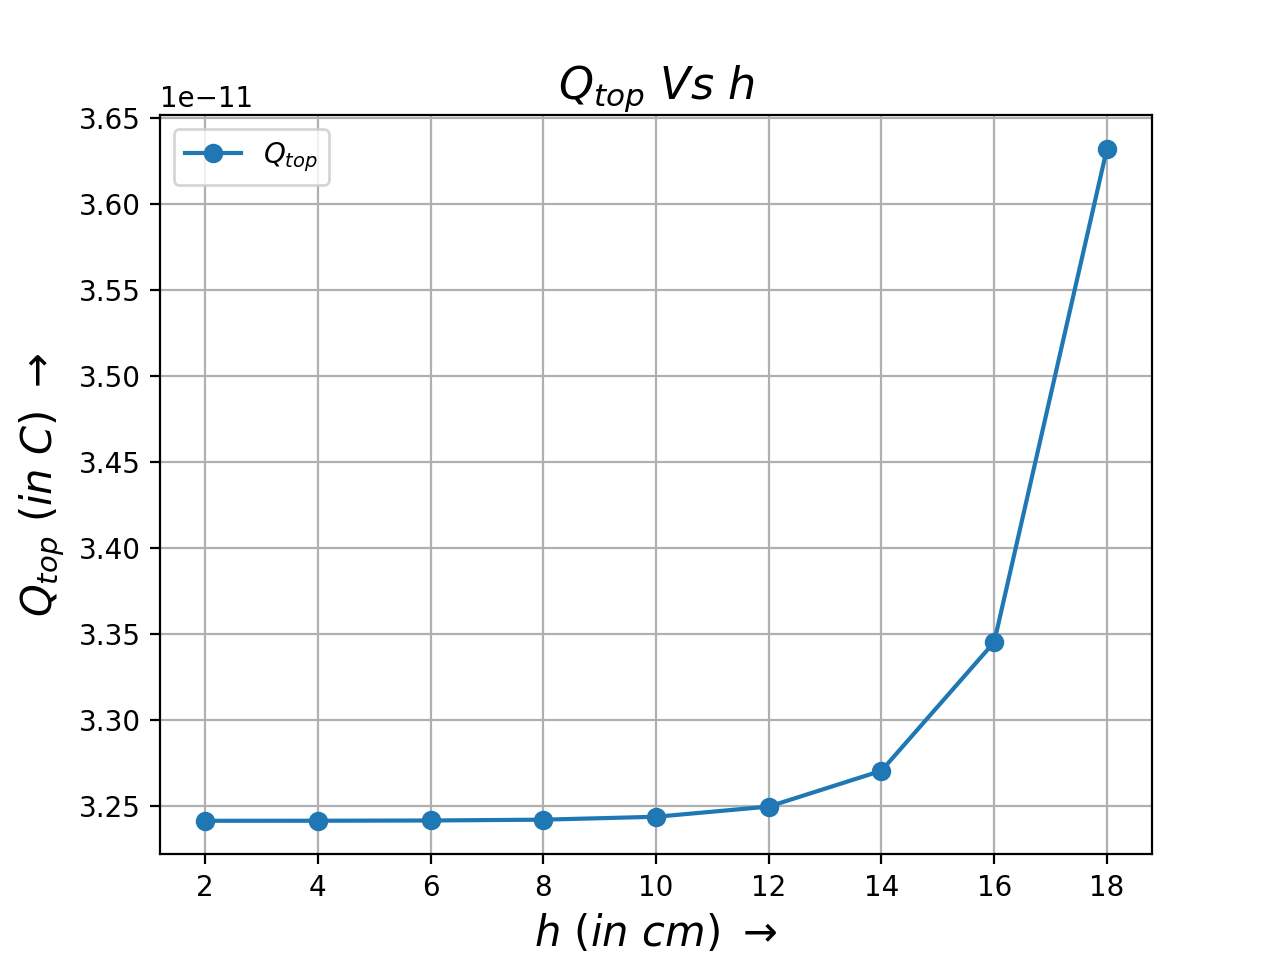
\includegraphics[scale=0.6]{qtop.png}
  \label{fig:qtop}
  \caption{Plot of $Q_{top}$ Vs $h$}
\end{figure}
\begin{figure}[H]
  \centering
  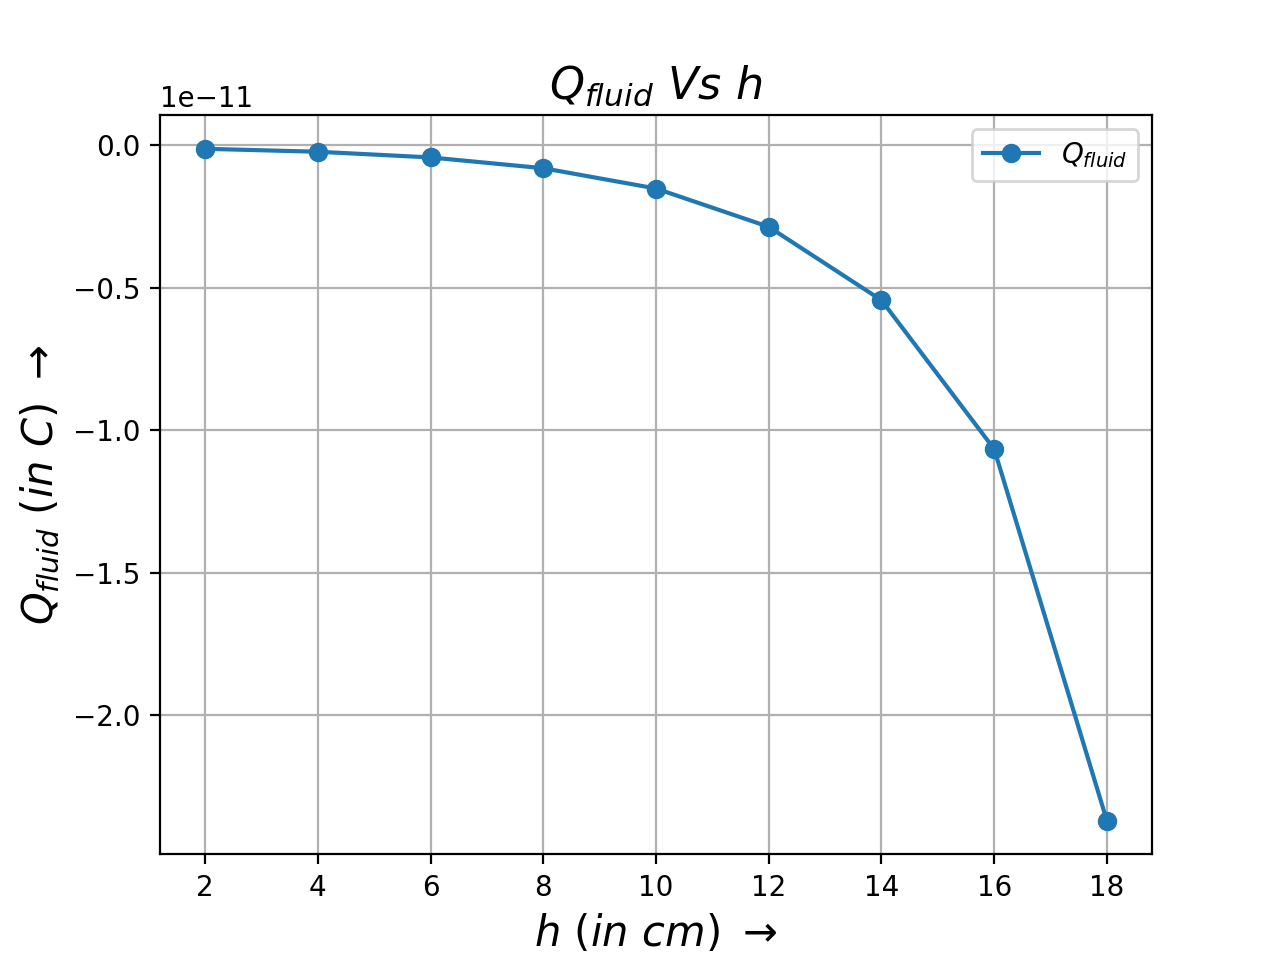
\includegraphics[scale=0.6]{qfluid.png}
  \label{fig:qfluid}
  \caption{Plot of $Q_{fluid}$ Vs $h$}
\end{figure}
Clearly, the plots do not represent a linear trend. It is neither exponential or a simple hyperbola (without any vertical shifting) as is seen from the below images :
\begin{figure}[H]
  \centering
  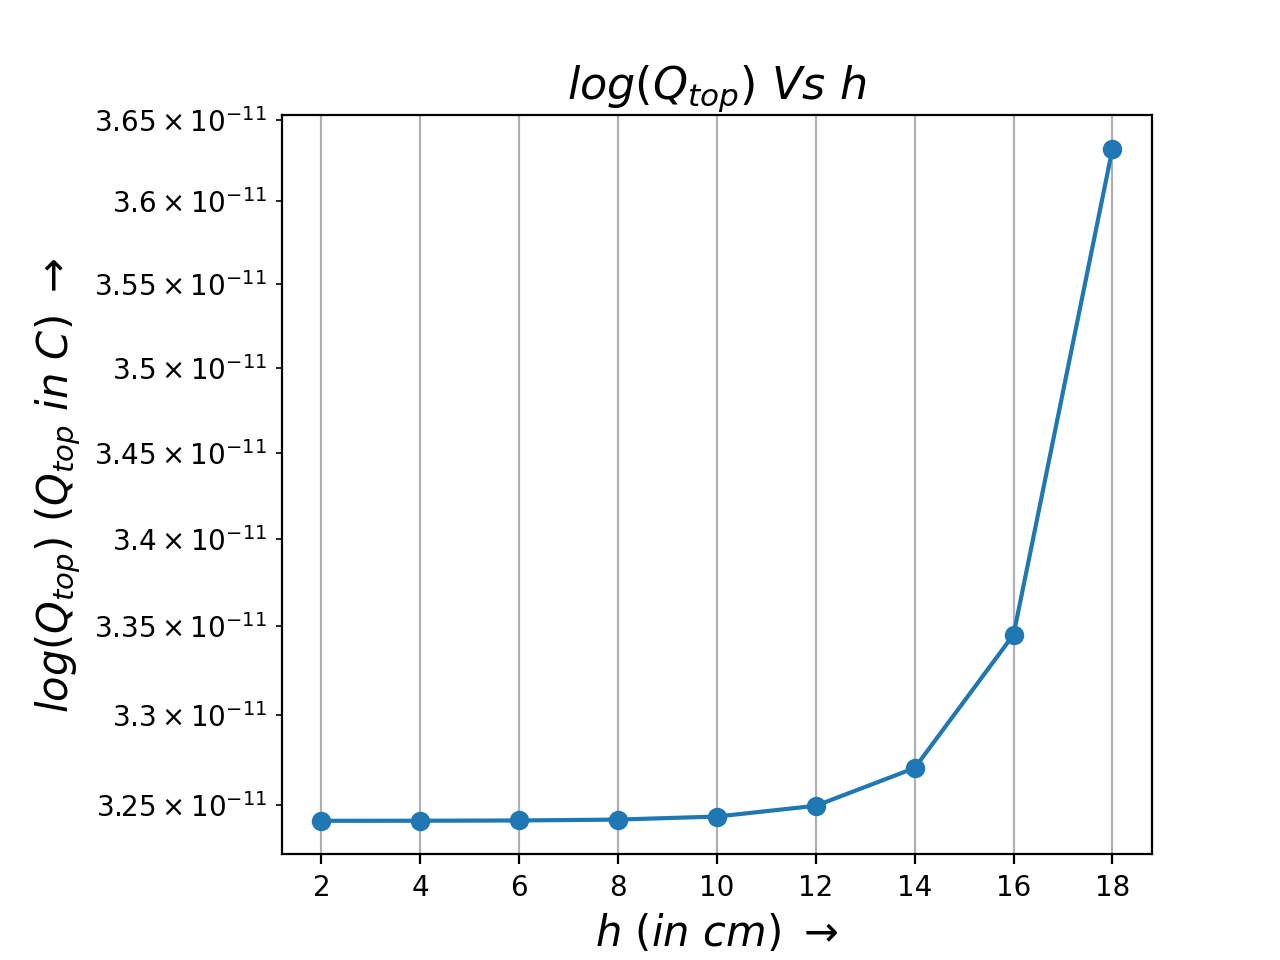
\includegraphics[scale=0.6]{qtop_semilog.png}
  \label{fig:qtop_semilog}
  \caption{Plot of $log(Q_{top})$ Vs $h$}
\end{figure}
\begin{figure}[H]
  \centering
  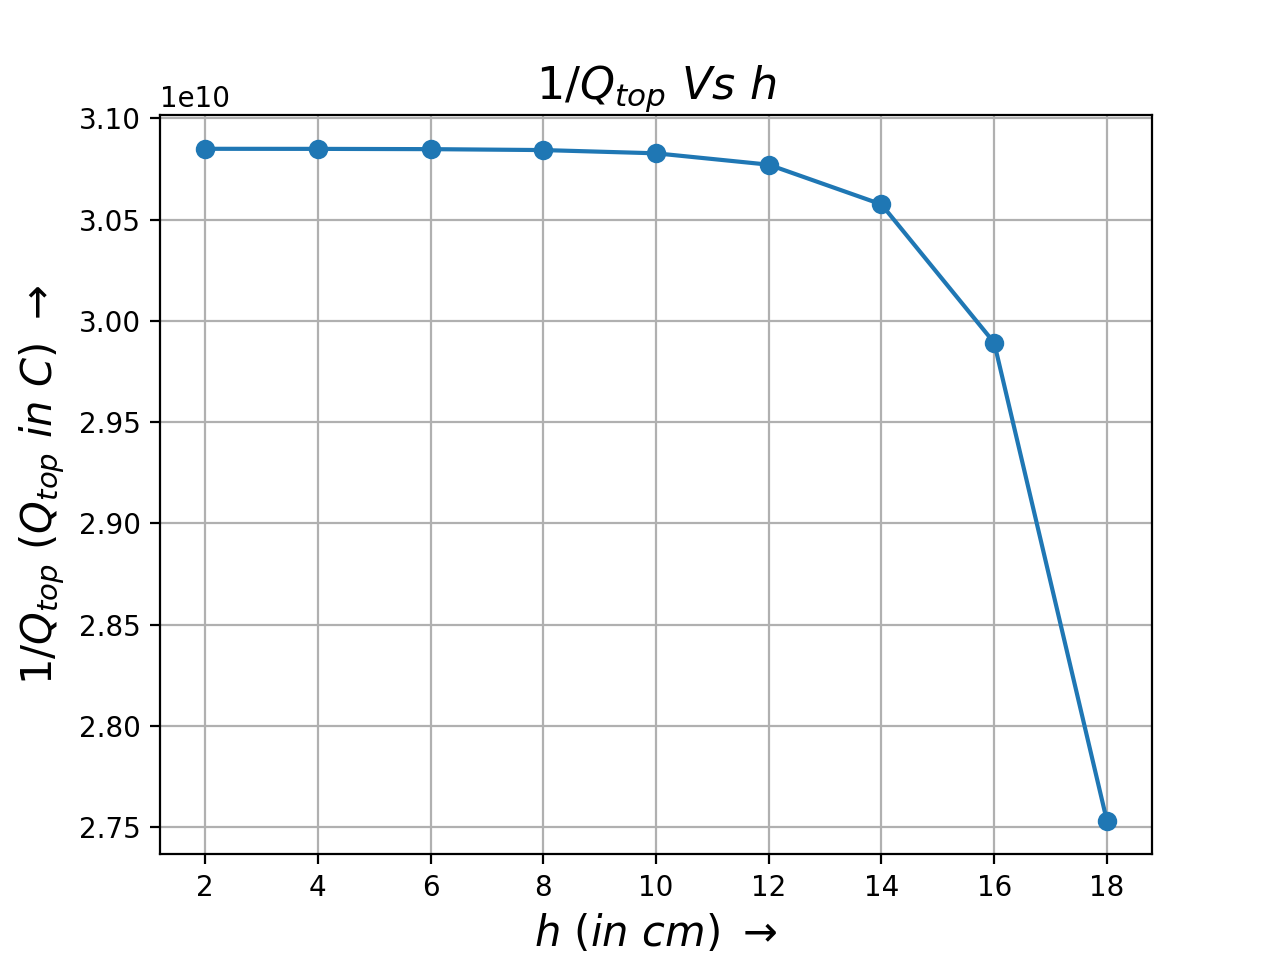
\includegraphics[scale=0.6]{qtop_hyper.png}
  \label{fig:qtop_hyper}
  \caption{Plot of $1/Q_{top}$ Vs $h$}
\end{figure}
This non-linearity might be because there is no reason for it to be linear.
\\
Consider an example similar to the given setup but much simpler, which is a parallel plate capacitor with plates separated by $d$ and partially filled with dielectric (with relative permittivity $\epsilon_r$) till height $h$.
It's capacitance is given by :
\[
  C = \frac{A\epsilon_o}{[d + h(\frac{1}{\epsilon_r} - 1)]}
\]
Since $Q = CV$ and V = 1 volts here, $Q = C$ which means $Q$ Vs $h$ varies as a hyperbolic function shifted in $h$.
Hence, $Q$ doesn't vary linearly with $h$ usually in capacitor and in our example too, it doesn't.

\subsection{Part F - Electric field at centre of mesh cells and Continuity of $D_n$ at m = k}
We define a function to calculate electric field at the centre of mesh cells for $h/Ly = 0.5$ by using $E_x$ and $E_y$ we calculated as one-sided derivative of potential.
The explanation for the same is mentioned in the comments :
\begin{minted}[tabsize = 4]{python3}
def ElectricField_Centre(phi):
  '''
      Function to calculate Ex and Ey at centre of mesh cells 
        (i.e) at (m+0.5,n+0.5)
      Takes in -
          phi : The potential grid
      -----------------------------------------------
      Returns -
          Ex_centre : Ex at centre of mesh cells
          Ey_centre : Ey at centre of mesh cells
  '''
  # Getting Ex and Ey
  Ex,Ey = ElectricField(phi)

  # Ex[m,n+1] finds Ex at (m,n+0.5). Ex at (m+0.5,n+0.5) would be 
  #   -(phi @ (m+0.5,n+1) - phi @ (m+0.5,n)) / dist
  # Since we don't know phi @ (m+0.5,n), we can approximate that as 
  #   average of phi @ (m,n) and phi @ (m+1,n)
  # Similarly for phi @ (m+0.5,n+1)
  # On rearranging the terms, we get Ex_centre[m+1,n+1] as 
  #   average of Ex[m+1,n+1] and Ex[m,n+1], which will be Ex at (m+0.5,n+0.5)
  Ex_centre = pl.zeros((M,N))
  Ex_centre[1:,1:] = 0.5 * (Ex[1:,1:] + Ex[:-1,1:])

  # Similarly Ey_centre[m+1,n+1] is average of 
  #   Ey[m+1,n+1] and Ey[m+1,n], which will be Ey at (m+0.5,n+0.5)
  Ey_centre = pl.zeros((M,N))
  Ey_centre[1:,1:] = 0.5 * (Ey[1:,1:] + Ey[1:,:-1])

  return Ex_centre,Ey_centre
\end{minted}
We calculate the $E_x$ and $E_y$ at centre of mesh cells (at (m+0.5,n+0.5)) using the function above, print them and also plot them as a quiver plot :
\begin{minted}[tabsize = 4]{python3}
####### Ex, Ey at (m+0.5,n+0.5) - at centre of mesh cells
Ex_centre,Ey_centre = ElectricField_Centre(phi)

# Printing the Ex and Ey at (m+0.5,n+0.5)
print('\n\nEx values at (m+0.5,n+0.5) :')
print(Ex_centre[1:,1:])

print('\nEy values at (m+0.5,n+0.5) :')
print(Ey_centre[1:,1:])

# x and y are the axes of the grid to make the quiver plot - 
#   coordinates of midpoint of the mesh cells
x_c = pl.arange(dist/2,Lx,dist)*100  # in cm
y_c = pl.arange(dist/2,Ly,dist)*100  # in cm
pl.figure(6)
pl.quiver(x_c,y_c,Ex_centre[1:,1:],Ey[1:,1:])
pl.xlabel(r'$X\ (in\ cm)\ \rightarrow$',size=15)
pl.ylabel(r'$Y\ (in\ cm)\ \rightarrow$',size=15)
pl.title('Electric field at centre of mesh cells',size=16)
pl.show()
\end{minted}
\begin{figure}[H]
  \centering
  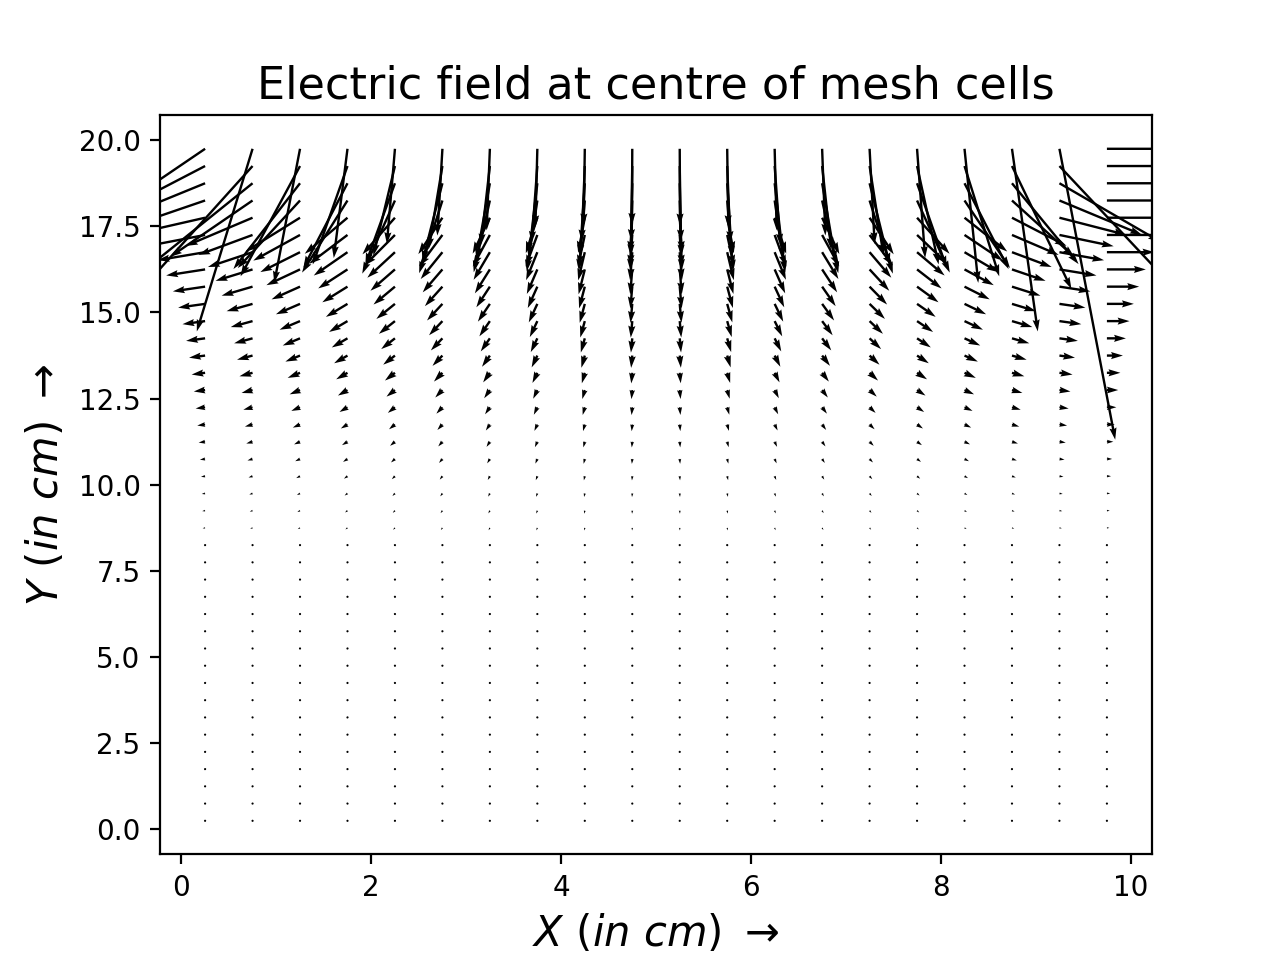
\includegraphics[scale=0.6]{EF_middle.png}
  \label{fig:EF_middle}
  \caption{Quiver plot of Electric Field at centre of mesh cells}
\end{figure}
The potential update \hyperref[eq:1]{here} we used had a different treatment for m = k row alone to make sure $D_n$ is continuous there.
The same is also verified by taking the $D_n$ which is $\epsilon E_y$ for the points (k+0.5,n) which are just above m = k,
and for the points (k-0.5,n) which are just below m = k. We check for continuity using the Left hand limit = Right hand limit method
and calculate percentage difference (as the numbers are originally small and just the difference won't confirm this) to check how close the values are :
\begin{minted}[tabsize = 4]{python3}
# Checking continuity of Dn at m = k
# Dn = e * En, where e = absolute permittivity of medium 
#   and En = Ey at the fluid surface m = k
# We are basically checking Dn just above and below are same =>
#   (Left hand limit = Right hand limit) => continuity
# I haven't multiplied by e_o since we are finding 
#   relative percentage difference which is a ratio

# Ey just above m = k (i,e) (k+0.5,n) => Ey_centre[k+1,1:]
# Ey just below m = k (i,e) (k-0.5,n) => Ey_centre[k,1:]
per_diff = abs((Ey_centre[k+1,1:]-e_r*Ey_centre[k,1:]) /
  Ey_centre[k+1,1:]).max() * 100  # percentage difference
print(f'\nThe relative difference between Dn \
  just above and below is nearly : {per_diff} %')
if per_diff < 0.1:
    print('Dn is continuous at m = k')
else :
    print('Dn is not continuous at m = k')
\end{minted}
We can see the output below :
\begin{figure}[H]
  \centering
  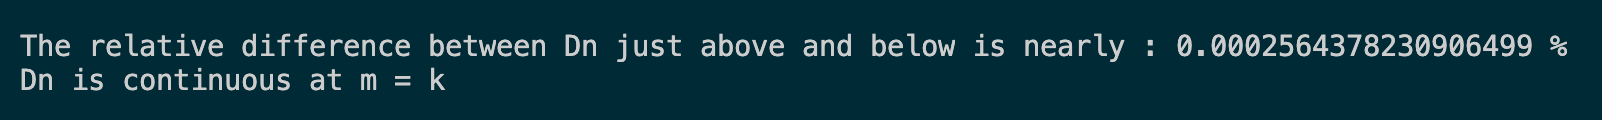
\includegraphics[scale=0.5]{cont_out.png}
  \label{fig:cont_out}
  \caption{Screenshot showing the output of $D_n$ continuity checking}
\end{figure}
I also plotted the electric field of the interior points, calculated using double-sided derivative of potential as a quiver plot :
\begin{minted}[tabsize = 4]{python3}
Ex_d = pl.zeros((M,N))
Ey_d = pl.zeros((M,N))
Ex_d[1:-1,1:-1] = -(phi[1:-1,2:] - phi[1:-1,:-2]) / dist
Ey_d[1:-1,1:-1] = -(phi[2:,1:-1] - phi[:-2,1:-1]) / dist
pl.figure(5)
pl.quiver(x,y,Ex_d,Ey_d)
pl.xlabel(r'$X\ (in\ cm)\ \rightarrow$',size=15)
pl.ylabel(r'$Y\ (in\ cm)\ \rightarrow$',size=15)
pl.title('Electric field at interior points of grid',size=16)
pl.show()
\end{minted}
\begin{figure}[H]
  \centering
  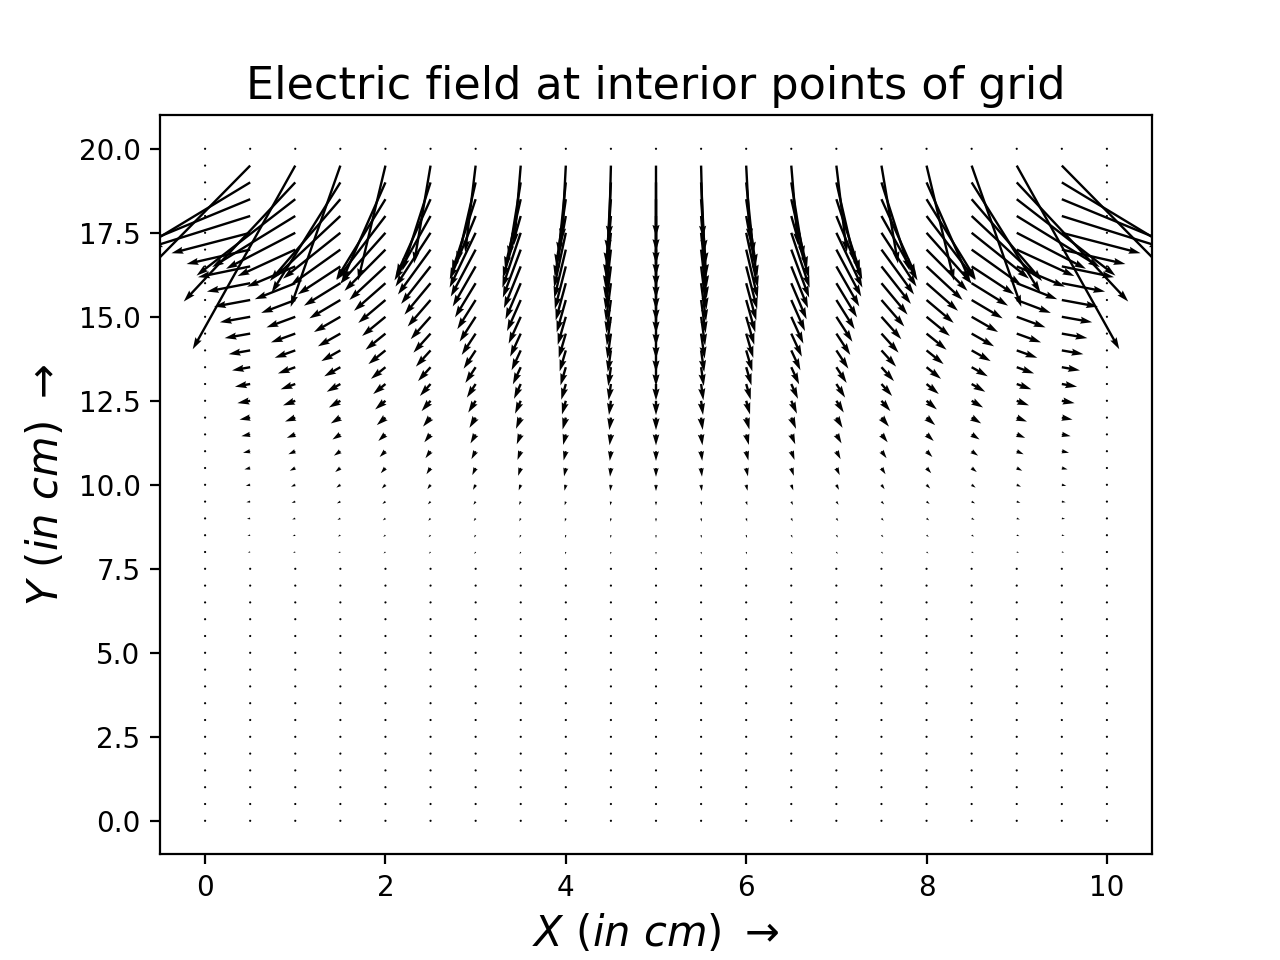
\includegraphics[scale=0.6]{EF_double.png}
  \label{fig:EF_double}
  \caption{Quiver plot of Electric Field calculated with double-sided derivative}
\end{figure}

\subsection{Part G - Checking validity of Snell's law}
We calculate the angle made by electric field with the normal to the fluid surface at m = k (i.e) along Y-axis,
by taking $\tan^{-1}(\frac{E_x}{E_y})$.\\
We do it for points just above m = k at (k+0.5,n) and just below m = k at (k-0.5,n),
so that we can calculate the change in angle of Electric field at m = k.
\begin{minted}[tabsize = 4]{python3}
# Using Ex_centre and Ey_centre from above part which calculated 
#   Electric fields along x and y axes at centre of mesh cells
# Angle made by electric field with normal (y-axis) at points
#   just below m = k (i.e) (k-0.5,n) - Theta1
angle_b = pl.arctan(pl.divide(Ex_centre[k,1:],Ey_centre[k,1:]))
# Angle made by electric field with normal (y-axis) at points 
#   just above m = k (i.e) (k+0.5,n) - Theta2
angle_t = pl.arctan(pl.divide(Ex_centre[k+1,1:],Ey_centre[k+1,1:]))

# Plot of change in angle of electric field (i.e) angle_t - angle_b
PLOT(x_c,angle_t-angle_b,r'$X\ (in\ cm)\ \rightarrow$',
  r'$Change\ in\ angle\ (in\ radians)\ \rightarrow$',pl.plot,'-o',
  "Change in angle of Electric Field at m = k",7)
pl.show()
# Uncomment the below line to print the change in angle of Electric field
# print(angle_t-angle_b)
\end{minted}
\begin{figure}[H]
  \centering
  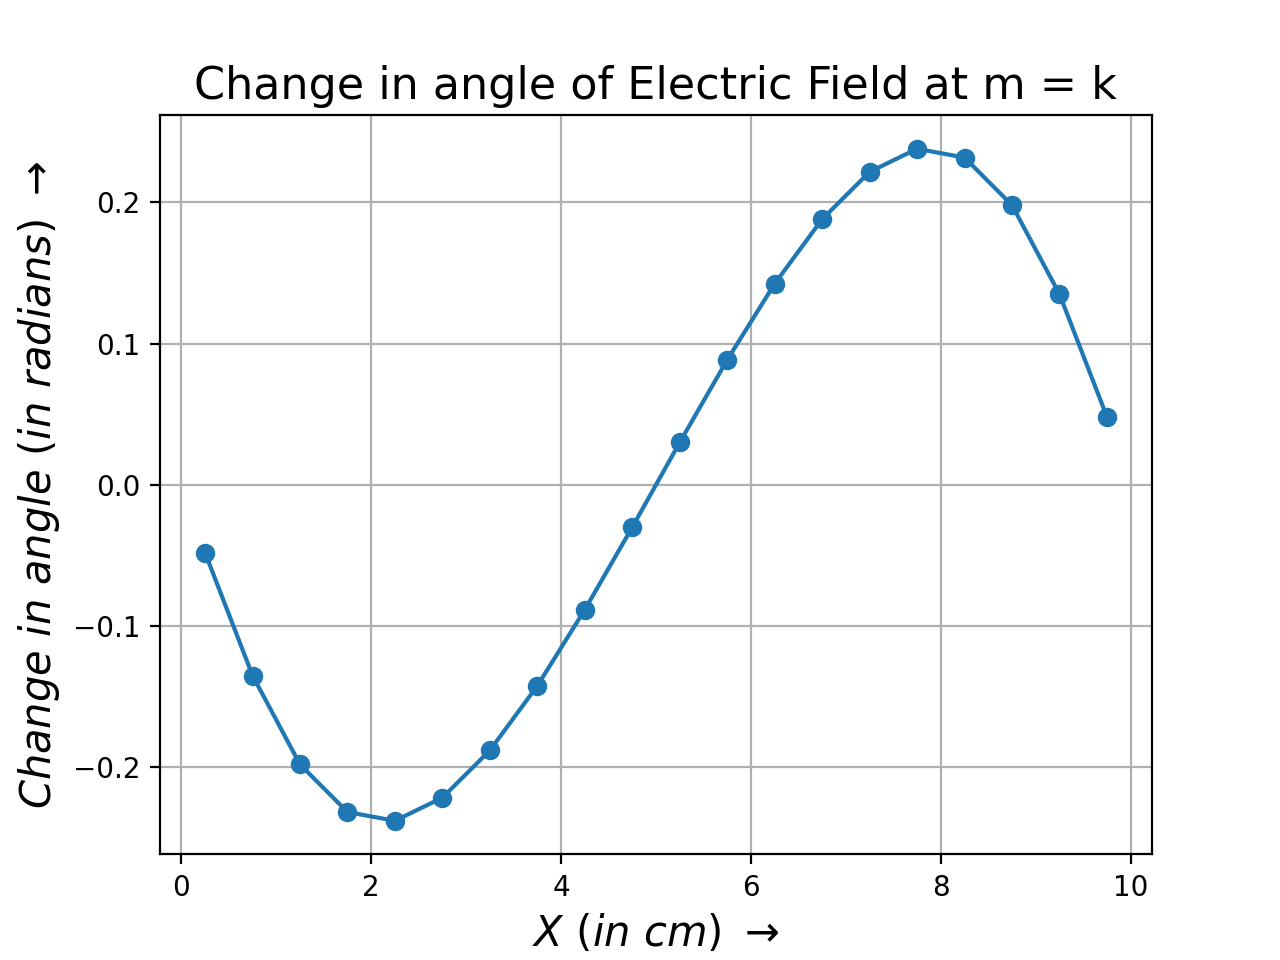
\includegraphics[scale=0.6]{angle_change.png}
  \label{fig:angle_change}
  \caption{Change in angle of Electric Field at m = k}
\end{figure}
To verify if the Electric field follows Snell's law when changing angle at the m = k fluid-air interface,
we plot $\frac{n_1\sin(\theta_1)}{n_2\sin(\theta_2)}$ at different points on m = k :
\begin{minted}[tabsize = 4]{python3}
# Leaving the constants behind since we are considering the ratio only
ratio =  (e_r**0.5 * pl.sin(angle_b)) / pl.sin(angle_t)  
# n1.sin(Theta1) / n2.sin(Theta2)
PLOT(x_c,ratio,r'$X\ (in\ cm)\ \rightarrow$',
  r'$\frac{n_1sin(\theta_1)}{n_2sin(\theta_2)}\ \rightarrow$',pl.plot,
  '-o',"Snell's law validity",8)
pl.show()
mean_ratio = ratio.mean()
std_ratio = ratio.std()
print(f'\nThe value of n1*sin(Theta1) / n2*sin(Theta2) has \
  mean : {mean_ratio} and standard deviation : {std_ratio}')
# The ratio has to be closer to 1 at all points for snell's law to be valid,
#   hence standard deviation of the ratio too has to be small apart from 
#   mean of the ratio being near to 1
if abs(mean_ratio-1.0) < 0.1 and std_ratio < 0.2:
    print("Snell's law is followed")
else :
    print("Snell's law is not followed")
\end{minted}
As mentioned in the code, the plot should have been a constant line at value 1 if 
Snell's law is valid, but the plot appears as bell-shaped :
\begin{figure}[H]
  \centering
  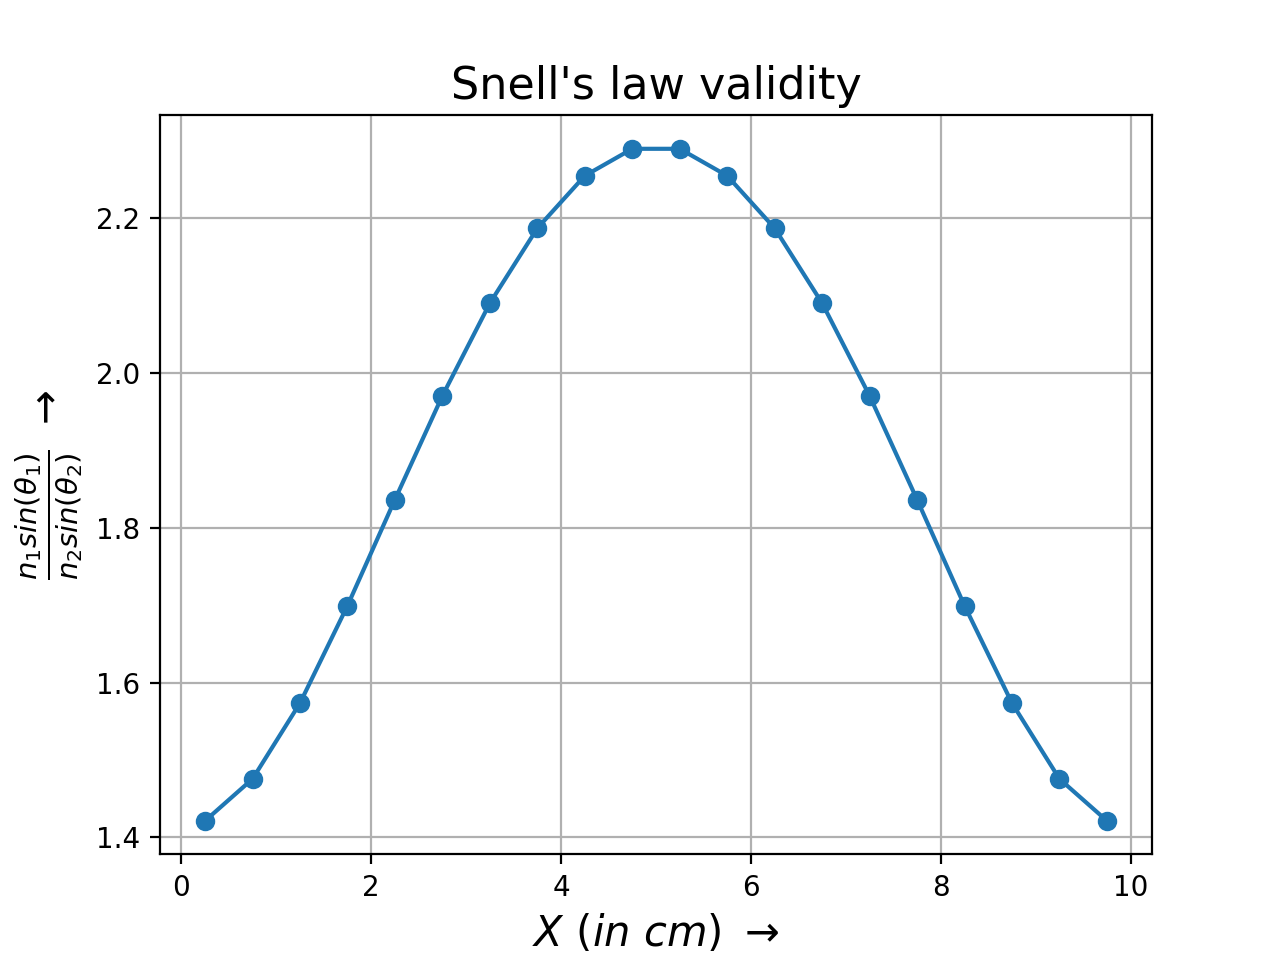
\includegraphics[scale=0.6]{snell.png}
  \label{fig:snell}
  \caption{$\frac{n_1\sin(\theta_1)}{n_2\sin(\theta_2)}$ Vs X}
\end{figure}
The output of the program can be seen below :
\begin{figure}[H]
  \centering
  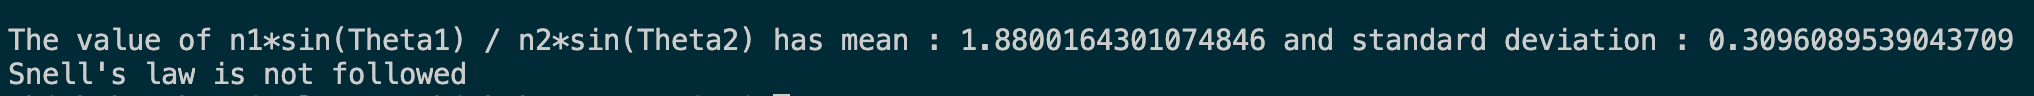
\includegraphics[scale=0.45]{snell_out.png}
  \label{fig:snell_out}
  \caption{Screenshot showing the mean and variance of the ratio we plotted}
\end{figure}
Clearly, Snell's law is not followed as shown by the plot and the mean value of ratio.
\\
The reason is that Snell's law was derived for Electro-magnetic waves where electric and magnetic fields sustain each other and propogate in space.
It is not exactly valid for electric field inside a capacitor. If it was so, there would not be any fringing of electric field lines in free space between capacitor plates at the edges,
where there is no interface at all. Electric field lines are not governed by the Snell's law, in general.

\section{Conclusions}
\begin{itemize}
\item We used iterative means to solve the 2-D Laplace equation and calculate potential efficiently using vectorized code.
\item We developed an algorithm to calculate height of fluid filled from the resonant frequency.
\item We obtained the electric field using numerical gradient of Potential.
\item We verified the continuity of $D_n$ at the fluid-air interface.
\item We observed that $Q_{top}$ and $Q_{fluid}$ do not vary linearly with $h$ in this capacitor setup.
\item We observed that Snell's law is not followed by the electric field at the interface.
\end{itemize}

\end{document}